\section{Testing of Causal Graphs}
\label{sec:graph-testing}

\subsection{Description}
\label{sec:testing-description}

\subsubsection{Testing observable assumptions}
\label{sec:observable-tests}
In the last section, we reviewed a process for creating an initial causal graph using expert opinion.
Critically, after drafting a causal graph, we should immediately test it against empirical data.
This is important because, if our graph captures inaccurate assumptions about the data generating process, then we have no reason to think that our conclusions from using the graph will be accurate.

To test our causal graphs against data, we will first test the implications of our graph that involve observable variables only.
We will defer the task of testing implications that involve unobserved / latent variables to later in this subsection.
For now, recall our discussion in Section \ref{sec:graph-overview} about the two basic implications of causal graphs: marginal independence and conditional independence.
In both cases, direct testing of marginal or conditional independence amongst nodes in the causal graph may be difficult.
Indeed, there are no direct tests of conditional independence that can detect all types of dependence, especially for continuous variables \citep{bergsma_2004_testing, shah_2020_hardness}.

As a result of this hardness, there are a myriad of research efforts aimed at testing conditional independence.
These efforts rely on additional assumptions about the variables or the test statistic itself.
Some researchers proceed under the assumption that one has access to an approximation of the conditional distribution of $X \mid Z$ \citep{candes_2018_panning, berrett_2019_conditional}.
Other researchers designed conditional independence tests for general cases, assuming smoothness of the underlying data distributions and assuming accurate estimation of the distribution of the test statistic under the null hypothesis of conditional independence (e.g. \citet{zhang_2012_kernel, strobl_2019_approximate}).

Different from (but not excluding) these approaches, we will take an easier and less decisive route.
If a pair of variables have conditionally or marginally independent distributions, then their statistical moments will also be conditionally or marginally independent.
Accordingly, we will not test for marginal or conditional independence in distribution.
We will instead perform a more tractable test for marginal or conditional independence in means.
If the variables in question are not conditionally or marginally independent in their means, then we know they are not independent in their distributions.
Conversely, even if a set of variables are marginally or conditionally independent in their means, this \textbf{does not} imply that the variables are independent in distribution.

This approach of indirectly assessing distributional independence by testing mean independence is not new.
The following papers have all proposed and implemented such an idea: \citet{burkart_2017_predictive, chalupka_2018_fast, inacio_2019_conditional}.
For conditional independences, the crux of the approach is to predict $Y$ based on $X$ and $Z$.
Then, compare against a prediction of $Y$ based on a resampled value of $X$ and the original $Z$.
If $Y$ is mean-independent of $X$ given $Z$, i.e. $E \left[ Y \mid X, Z \right] = E\left[ Y \mid Z \right]$, then the predictive power of a model with resampled $X$ should resemble the predictive power of a model with the original $X$.
After all, in both cases, the conditional expectation of $Y$ is independent of one's $X$ values (real or resampled).
When assessing marginal independencies, one removes $Z$ from the models for the expectation of $Y$ and proceeds as described.

Note that as with the case of testing distributional independence, testing mean independence still requires researchers to make choices.
We have to select models for $E \left[ Y \mid X, Z \right]$ and $E\left[ Y \mid Z \right]$, respectively, for testing conditional and marginal mean-independence.
We also have to choose the performance statistic (e.g. $R^2$, log-likelihood, etc.) to compare these models.
Lastly, we also have to select a resampling method.
In particular, how (if at all) will our resampling strategy account for the possible dependence between $X$ and $Z$?

% State the choices made in this work.
% Provide some discussion of the alternatives and the effects of different choices.
For our demonstration, we made the following choices.
First, we used linear regressions to model $E \left[Y \mid X, Z \right]$ and $E \left[ Y \mid Z \right]$.
Second, we used $R^2$ as our test statistic for judging the predictive performance.
Third, we resampled $X$ without replacement, keeping the length of the resampled vector equal to the length of the original vector.
In other words, we permuted $X$.
Finally, we visualized our tests by encoding our observed test-statistic as a vertical line and by plotting the kernel density estimate of our test statistic's distribution.

Our rationale for these choices are as follows.
In our dataset, most of our explanatory variables were continuous (at least in theory).
Accordingly, $R^2$ seemed a sensible performance metric for a model of the conditional expectation of a continuous random variable.

In contrast to our choice of performance metric, we chose our conditional expectation models and resampling methods through empirical testing.
In particular, we created simulations to assess our mean-independence testing procedure.
We assessed the performance of our mean-independence testing procedures using simulations where $Y \leftarrow Z \rightarrow X$ and $X$ either did or did not cause $Y$.

Of particular importance were our simulations under the null hypothesis where $X$ was conditionally independent of $Y$.
Our initial simulations used random forests as our conditional expectation models and permutations as resampling methods.
Random forests are a non-parametric method that would allow us to have less fear of model misspecification, and permutations are easy to implement.
However, under the null hypothesis, the random forest-based tests resulted in non-uniform p-values.
Such non-uniform p-values makes it harder to a-priori reject a false model \citep{gelman_2013_two}.
When we switched from the combination of random forests and permutations to linear regressions and permutations, our p-values were indeed empirically, uniformly distributed.
Moreover, we still retained high power.

We do not claim that these choices for assessing mean independence will always be appropriate.
Indeed, one should assess one's tests on simulated data that resembles one's real data.
For our illustrative purposes though, the combination of linear regressions, permutations, and $R^2$ resulted in adequate tests of marginal and conditional mean-independence.

\subsection{Demonstration}
\label{sec:testing-demonstration}

\begin{figure}
   \centering
   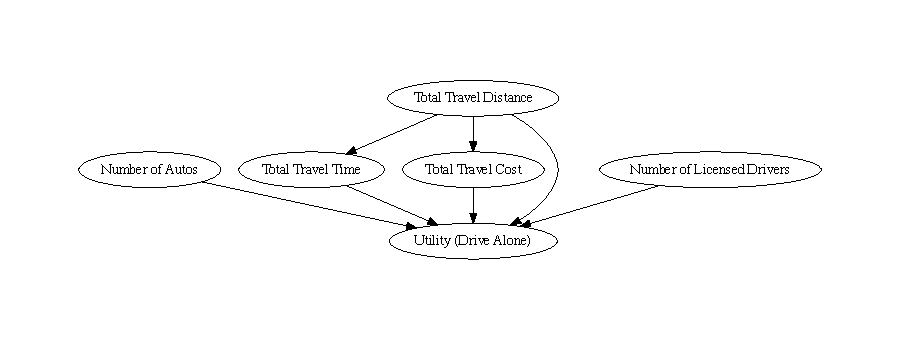
\includegraphics[width=0.85\textwidth]{drive-alone-utility-graph}
   \caption{Expository causal graph of drive alone utility}
   \label{fig:graph-for-testing}
\end{figure}
% Illustrative causal graph
To demonstrate the testing procedures described above, we used the causal graph in Figure \ref{fig:graph-for-testing}.
This causal graph shows a set of hypothesized causal relationships between variables thought to contribute to the utility of the drive-alone travel alternative in our dataset.
As drawn, this graph encodes multiple marginal and conditional independence assumptions.
Luckily, tools such as Daggity \citep{textor_2016_robust} can infer all independencies based on one's graph.
For didactic purposes, however, we focused our attention on two particular independence assumptions.

First, we tested the assumption of marginal independence between the number of licensed drivers and the number of automobiles in a household.
A-priori, we assign low probability to this independence.
Generally, we expect the number of automobiles to be positively related to the number of licensed drivers in a household.
Secondly, we tested the assumption that travel cost was independent of travel time, conditional on travel distance.
Unlike the previous independence assertion, this conditional independence is a-priori more credible.
In both cases, we will test our assumptions using the previous subsection's procedures.

% Marginal testing results
\begin{figure}
   \centering
   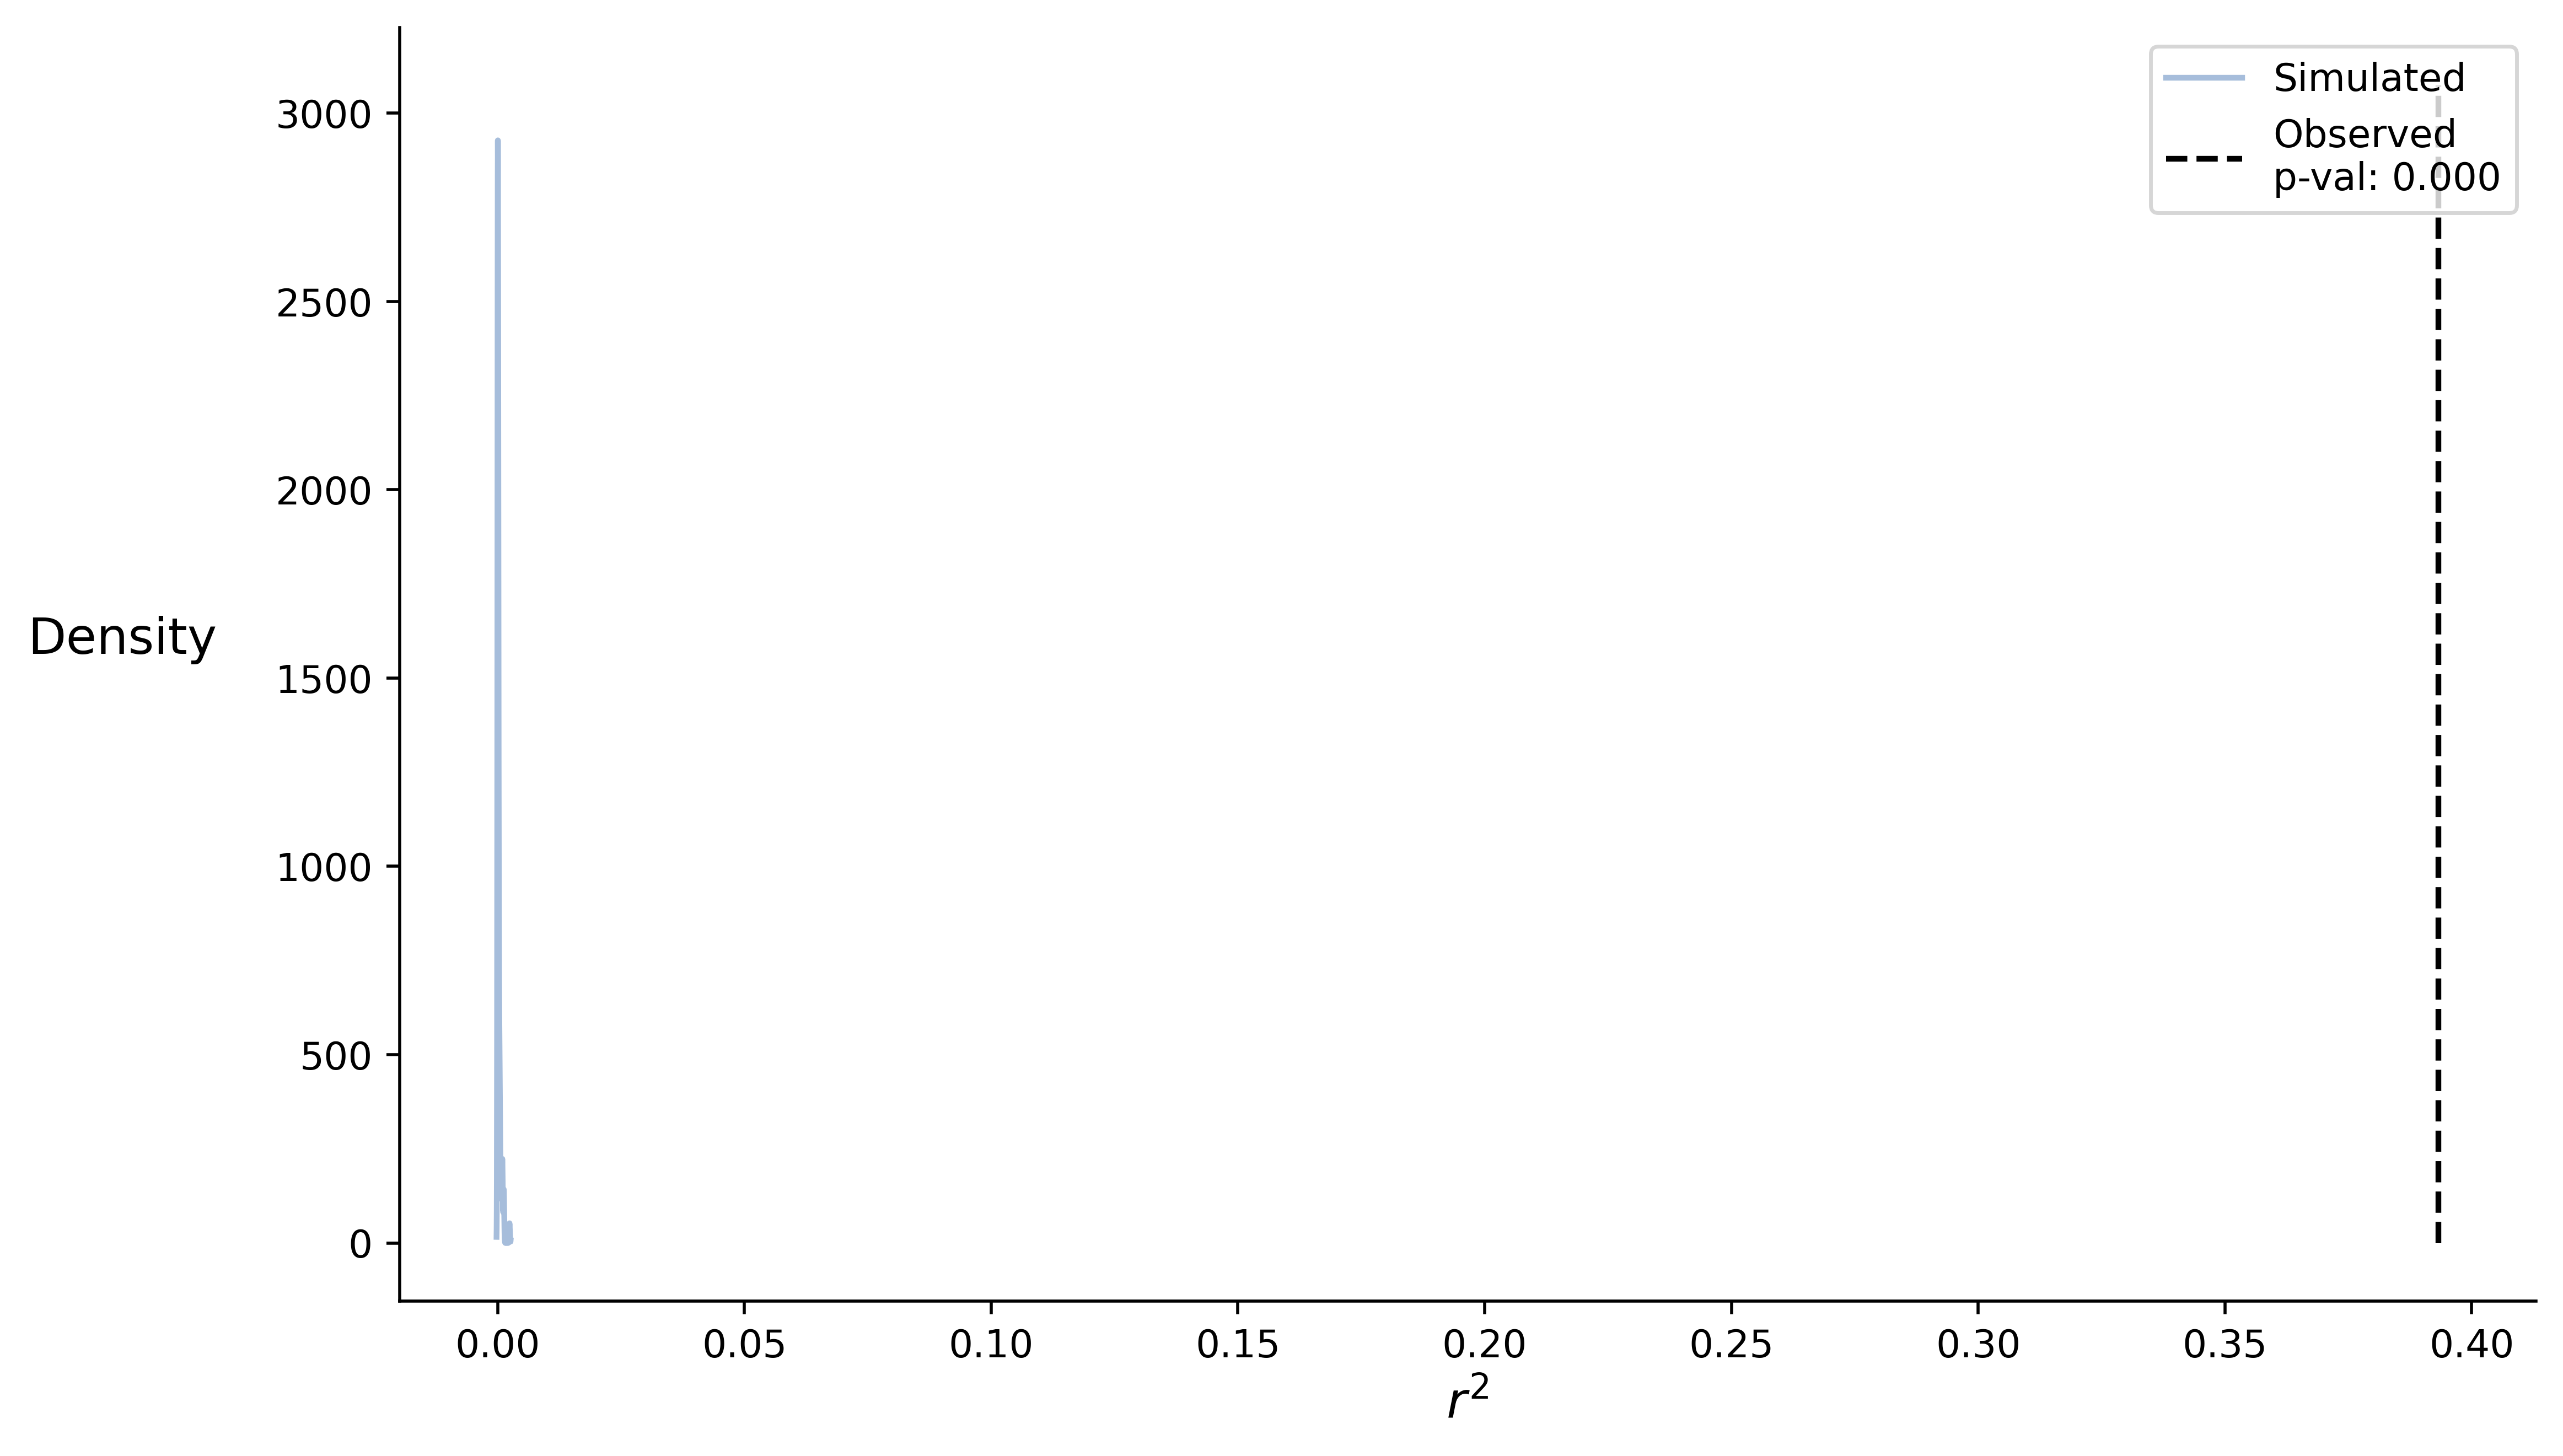
\includegraphics[width=0.5\textwidth]{mit--num_drivers_vs_num_autos.png}
   \caption{Marginal independence test results for the number of cars and licensed drivers in a household}
   \label{fig:marginal-independence-test}
\end{figure}

In particular, Figure \ref{fig:marginal-independence-test} shows the results of using permutation, linear regression, and $R^2$ to test the hypothesis of marginal independence between the number of automobiles and the number of licensed drivers in a household.
The empirical p-value of 0 confirms that the observed data is unlikely given the null-hypothesis of marginal, mean-independence.
More specifically, when regressing the number of licensed drivers in a household on the number of cars in that household, one achieves an $R^2$ near 0.4.
In contrast, when permuting the number of cars in the household and re-estimating the regression, the distribution of p-values concentrates around 0.
This plot visualizes the fact that---through the lens of our chosen test statistic ($R^2$), linear regression model, and permutation-based resampling strategy---data generated under an assumption of marginal mean-independence does not ``look like'' the observed data.
Accordingly, we should consider the weaker assumption of marginal dependence.
This relaxation may contain data-generating assumptions that better reflect our observations.

% Conditional testing results
\begin{figure}
   \centering
   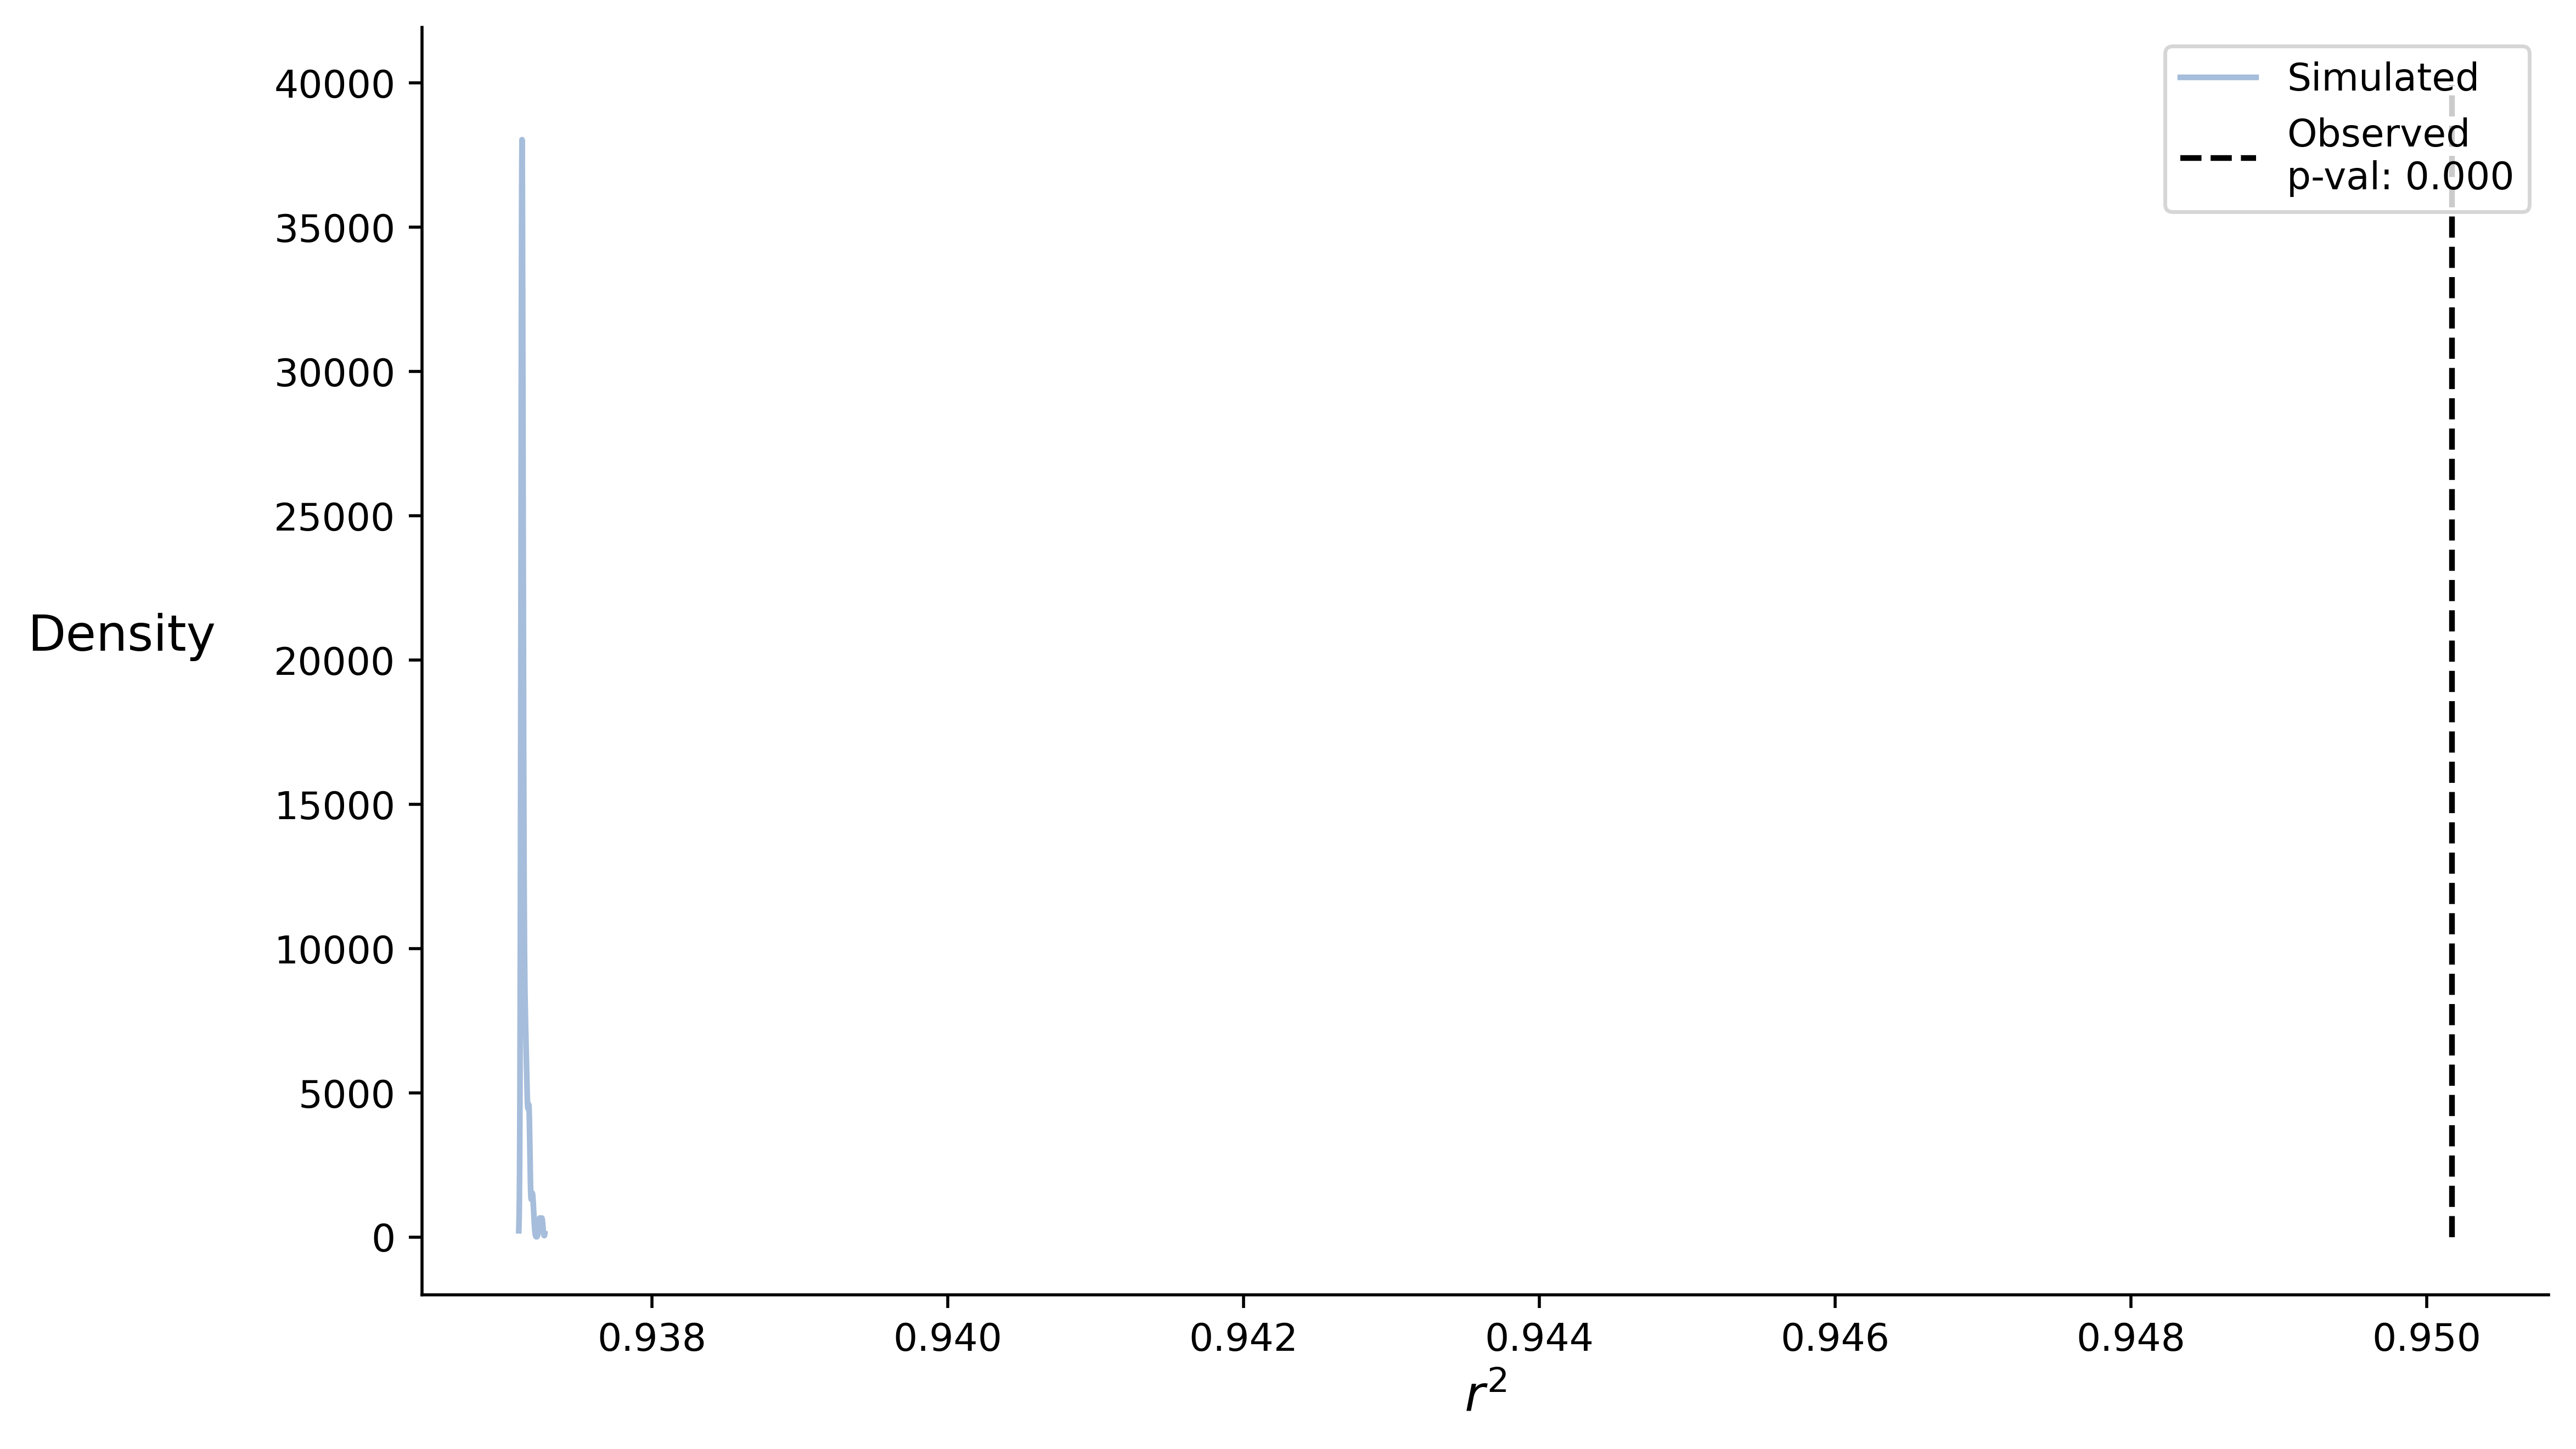
\includegraphics[width=0.5\textwidth]{cit--time_vs_cost_given_distance}
   \caption{Conditional independence test results for travel time and travel cost given travel distance}
   \label{fig:conditional-independence-test}
\end{figure}
In Figure \ref{fig:conditional-independence-test}, we have an analogous visualization of a conditional independence test.
Here, we test the hypothesis that travel time is mean-independent of travel cost, conditional on travel distance.
To execute this test, we model the conditional expectation of travel time as a linear function of travel cost and travel distance.
As with the marginal independence test results, the $R^2$ of the model using the observed values of travel cost are greater than the model's $R^2$ using any simulated datasets.
Again, this means that the $R^2$ using observed data is unlikely given our method of sampling from the null distribution of $R^2$ given conditional, mean-independence of travel time and travel cost.

As before, these results suggest conditional dependence between our variables of interest.
In particular, we should investigate how travel time and travel cost relate, conditional on travel distance.
Why might this be the case?
Does travel time cause travel cost when driving alone?
Does travel cost cause travel time while driving alone?
Does some other set of variables (potentially unmeasured) cause both travel time and travel cost?

Thinking through these questions, we can immediately think of latent variables that cause both travel time, travel cost, and the choice, even after conditioning on one's travel distance.
For example, consider whether one drives alone over the San Francisco Bay Bridge.
If one crosses the bridge, then traffic delays will likely increase one's travel time.
Moreover, if one crosses the bridge, then one's travel cost is higher due to tolls that one must pay.
And finally, if one takes a toll lane to get across the bridge faster, then one also pays a higher price.
Overall, intuitive explanations exist for conditional dependence between travel time and travel cost.
These explanations suggest particular relationships to analyze and particular variables, such as bay bridge crossings, to include in one's mode choice (i.e. outcome) model.

\subsubsection{Testing assumptions involving latent variables}
\label{sec:latent-tests}
% Describe latent variable testing
Now that we have described testing with observable variables, we can more easily describe conditional independence tests that involve unobserved (i.e., latent) variables.
Indeed, when dealing with observational data, we will frequently find ourselves not having observed all variables that are of interest.
Nevertheless, we still wish to test whether our data contradicts our graph.
One way to directly extend our conditional independence testing to account for latent variables is to adopt a missing data perspective and impute the latent variables from a prior distribution.
In particular, we can generalize our previous tests as follows.

First, we can consider expanding our test.
Instead of performing one test with a set of observed $X$, observed $Y$ and observed $Z$, we perform tests of observed $X$, observed $Y$, and imputed $Z$.
This recasts the randomness underlying the null-distribution in our original test statistic of $R^2$ as a function of our permutation of $Y$ and our imputation of $Z$.
Here, we impute $Z$ by sampling from the prior or posterior distribution of $Z$, depending on whether we're testing independencies before or after performing inference on our model's parameters.
Moreover, we'll now compute this test's p-value by averaging over the permutations and imputations.
Specifically, our p-value will be
\begin{equation}
E_{\textrm{samples, permutations}} \left[ \mathbb{I} \left \lbrace R^2 \left( X, Y, Z_{\textrm{sampled}} \right) <  R^2 \left( X_{\textrm{sampled}}, Y_{\textrm{sampled}} ^{\textrm{permuted}}, Z_{\textrm{sampled}} \right) \right \rbrace \right]
\end{equation}
where $\mathbb{I}$ represents the indicator function that equals one if the condition inside its braces is true and zero otherwise.
For reference, this is the same as the p-value for test statistics (or discrepancies) defined in \citet[Eq. 7]{gelman_1996_posterior}.

\begin{figure}
   \centering
   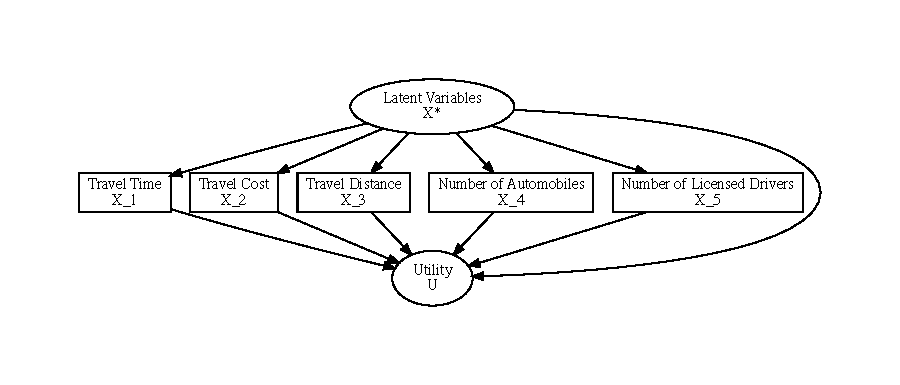
\includegraphics[width=0.85\textwidth]{deconfounder-causal-graph}
   \caption{Causal graph from applying the deconfounder algorithm \citep{wang_2019_blessings} to our dataset.}
   \label{fig:deconfounder-graph}
\end{figure}

\begin{figure}
   \centering
   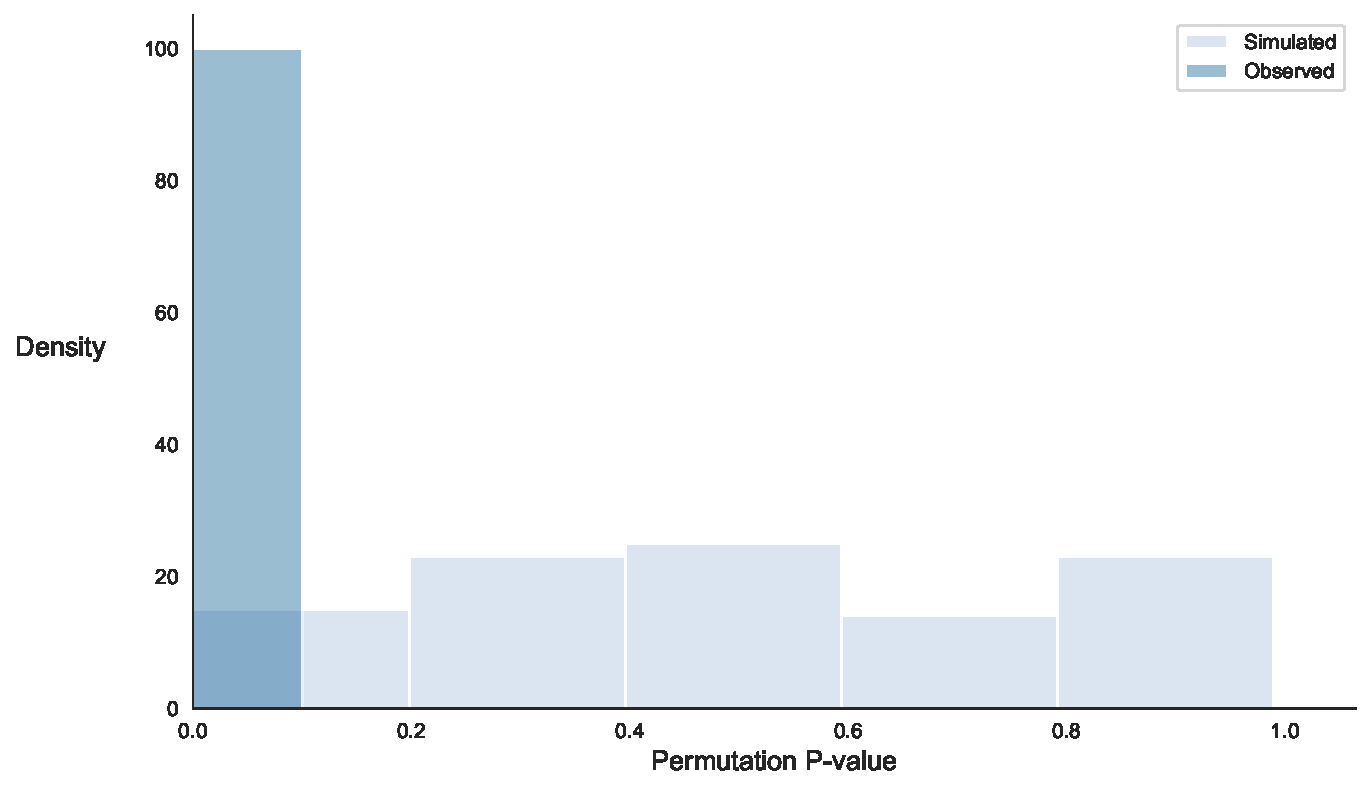
\includegraphics[width=0.5\textwidth]{latent-drivers-vs-num-autos}
   \caption{Results of testing that the number of drivers is independent of the number of automobiles in the household, conditional on the latent variable.}
   \label{fig:latent-cit-results}
\end{figure}

Lastly, note that our ``observed'' test statistic is itself a random variable: it depends on the imputed values of $Z$.
Because we now have a distribution of observed test statistics, we change our visualization method.
Instead of plotting a single line versus a distribution, we now plot two distributions against one another.
We first plot the distribution of ``observed'' test statistics that we computed using the observed $X$, observed $Y$ and imputed $Z$ values.
Then, we plot the distribution of ``sampled'' test statistics using prior samples of $\left( X, Y, Z \right)$ as a reference.
Here, we have one value per imputed vector $Z$ in both the observed and sampled distributions.
However, for the distribution of ``sampled'' test statistics, we marginalize over permutations of $Y$ since this distribution represents the null hypothesis of conditional or marginal independence.

That last paragraph may have been confusing, so we'll walk through an example.
Here, we apply the deconfounder algorithm of \citet{wang_2019_blessings} to our data.
In particular, Figure \ref{fig:deconfounder-graph} shows the deconfounder's assumed causal graph.
Note, we describe this application more thoroughly in Section \ref{sec:latent-confounding}.
For now, we present the graph to highlight the assumptions that we will test.
Specifically, we'll examine the assumption that the observed number of licensed drivers in a household is independent of the observed number of automobiles in that household, conditional on the latent variable $X^{*}$.

Figure \ref{fig:latent-cit-results} shows the result of following the aforementioned testing procedures for assumptions involving latent variables.
From the Figure, we see that the distribution of ``observed'' test statistics clusters around zero while the distribution of ``sampled'' test statistics is closer to uniform.
This result highlights the fact that (generally) there is ``no free lunch'': our approach to testing assumptions involving latent variables has its drawbacks.
In particular, these tests are sensitive to assumptions about the joint prior distribution, $P_{\textrm{prior}} \left( X, Y, Z \right)$.

If, as in this case\footnote{Details of the prior predictive checks that show prior-data mismatch are not shown due to space constraints. Please see \url{https://github.com/hassan-obeid/tr_b_causal_2020/blob/master/notebooks/final/_04-tb-testing-your-causal-graph.ipynb}}, the observed data $\left( X, Y \right)$ is unlikely under the joint prior distribution $P_{\textrm{prior}} \left( X, Y, Z \right)$ then the conditional independence test is likely to fail.
As always, the failing test indicates that the observed data is unlike the simulated data used to make the reference distribution.
Unfortunately, we are unsure of how much dissimilarity comes from conditional independence violations.
The observed data can differ distributionally from the simulated data in many ways.
This highlights the need for extensive prior predictive checking of one's assumed joint prior, $P_{\textrm{prior}} \left( X, Y, Z \right)$, \textit{before} using conditional independence tests on causal graphs with latent variables.

\subsection{Additional techniques}
\label{sec:testing-addendum}

The methods presented in this section test independence assertions using one's dataset.
While perhaps the most accessible strategy for testing one's causal graph, other techniques apply as well.
For instance, \citet{pitchforth_2013_proposed} proposed a checklist of qualitative questions for one's causal graph.
Answering these questions should increase the trustworthiness of one's graph.
Alternatively, there are other quantitative tests of one's causal graph that were not explored in this section.

For instance, causal graphs encode assumptions about the number of independent variables in one's data.
The independent variables are the parentless-nodes in one's graph.
Crucially, each graph assumes a particular number of such parentless-nodes.
To test this assumption we first estimate our data's ``intrinsic dimension.''
Then, we test whether the intrinsic dimension equals the number of parentless-nodes in our graph.
For more information on estimating the intrinsic dimension of a dataset, see \citet{camastra_2016_intrinsic, song_2019_identification}.
Additionally, see \citet{chenwei_2019_likelihood} for an extension of this idea when we cannot rule out unobserved confounding.

% Test vanishing tetrads / t-separation
Another empirical implication of one's causal graph is the existence of so-called ``vanishing tetrads'' \citep{spearman_1904_general}.
This term signifies that the difference between the product of two particular pairs of covariances must be zero.
As stated, this implication of one's causal graph is hard to intuitively understand.
However, one can graphically determine the existence of vanishing tetrads and determine which variables are part of these tetrads.
Then, one can estimate the necessary covariances and test to see if their difference of products is indeed unlikely to be zero.
Such a test is yet another way to empirically determine whether one's graph is incompatible with one's dataset.
For the original theorems proving that tetrads can be graphically identified and characterized, see \citet{shafer_1996_vanishing} and references therein.
For a more detailed and intuitive explanation of the graphical criterion for vanishing tetrads, see \citet{thoemmes_2018_local}.

% Test functional inequalities / constraints, i.e. entropy constraints / inflation technique
Finally, we note that there are still a whole host of other techniques for testing one's causal graphs.
Many of these remaining techniques are useful when one's causal graph contains unobserved (i.e., latent) variables.
On one hand, we can use ``triad constraint'' tests that test independence between ``pseudo-residual'' values and one's explanatory variables \citep{cai_2019_triad}.
Results from these tests are useful for judging how unobserved variables in our graph relate to each other and to our observed variables.

Relatedly, one can make use of constraints on entropies of our observed variables instead of independencies.
The idea is that differing latent variable graphs imply differing entropies in our observed variables.
Accordingly, we test for these entropies and constraints.
For more information and examples, see the literature about:
\begin{itemize}
  \item inequality constraints, e.g. \citet{tian_2002_testable, kang_2006_inequality, ver_2011_sequence}
  \item information inequalities, e.g. \citet{chaves_2014_inferring}
  \item entropic inequalities, e.g. \citet{chaves_2014_causal}
  \item the inflation technique, e.g. \citet{wolfe_2019_inflation, navascues_2020_inflation}
\end{itemize}
